\documentclass[conference]{IEEEtran}
\IEEEoverridecommandlockouts
% The preceding line is only needed to identify funding in the first footnote. If that is unneeded, please comment it out.
\usepackage{cite}
\usepackage{amsmath,amssymb,amsfonts}
\usepackage{algorithmic}
\usepackage{algorithm}
\usepackage{graphicx}
\usepackage{textcomp}
\usepackage{float}
\usepackage{xcolor}
\def\BibTeX{{\rm B\kern-.05em{\sc i\kern-.025em b}\kern-.08em
    T\kern-.1667em\lower.7ex\hbox{E}\kern-.125emX}}
\begin{document}

\title{Joint Optimization of Energy, Latency and Age of Information for MEC Task Offloading Using TLBO-HHO Algorithm\\
\thanks{Identify applicable funding agency here. If none, delete this.}
}

\author{\IEEEauthorblockN{1\textsuperscript{st} Given Name Surname}
\IEEEauthorblockA{\textit{dept. name of organization (of Aff.)} \\
\textit{name of organization (of Aff.)}\\
City, Country \\
email address or ORCID}
\and
\IEEEauthorblockN{2\textsuperscript{nd} Given Name Surname}
\IEEEauthorblockA{\textit{dept. name of organization (of Aff.)} \\
\textit{name of organization (of Aff.)}\\
City, Country \\
email address or ORCID}
\and
\IEEEauthorblockN{3\textsuperscript{rd} Given Name Surname}
\IEEEauthorblockA{\textit{dept. name of organization (of Aff.)} \\
\textit{name of organization (of Aff.)}\\
City, Country \\
email address or ORCID}
}

\maketitle

\begin{abstract}
Mobile Edge Computing (MEC) provides low-latency and energy-efficient computing services for resource-constrained mobile devices by deploying computing resources at the network edge. However, in multi-user scenarios, how to effectively make task offloading decisions while optimizing system energy consumption, latency, and information freshness remains a challenging problem. This paper proposes a hybrid metaheuristic algorithm (TLBO-HHO) that integrates Teaching-Learning-Based Optimization (TLBO) and Harris Hawks Optimization (HHO) to solve the task offloading and resource allocation optimization problem in MEC environments considering Age of Information (AoI). The main contributions include: (1) establishing a tri-objective optimization model considering energy consumption, latency, and AoI, using queuing theory to analyze task waiting time, and proving its NP-hardness; (2) designing a two-phase integrated TLBO-HHO fusion algorithm that balances global exploration and local exploitation through an adaptive switching mechanism; (3) experimental results show that compared to the original TLBO, GA, and GWO algorithms, TLBO-HHO improves fitness values by 65.2\%, 85.4\%, and 74.6\% respectively, while effectively reducing information staleness.
\end{abstract}

\begin{IEEEkeywords}
Mobile edge computing, task offloading, resource allocation, age of information, teaching-learning-based optimization, Harris hawks optimization, two-phase integration.
\end{IEEEkeywords}

\section{Introduction}
With the rapid development of Internet of Things (IoT) and 5G/6G communication technologies, the amount of data generated by mobile devices is growing exponentially. Mobile Edge Computing (MEC) provides an effective solution for delay-sensitive applications by deploying computing resources at the network edge~\cite{b1}. In MEC systems, task offloading decisions directly affect system performance and need to balance between energy consumption and latency. In recent years, with the increasing demand for real-time communication and real-time decision-making, Age of Information (AoI) has become an important metric for measuring system information freshness~\cite{b15}, and incorporating AoI optimization has become a research trend.

Existing research methods include convex optimization~\cite{b2}, game theory, deep reinforcement learning~\cite{b3}, and metaheuristic algorithms. However, single metaheuristic algorithms have inherent defects: Genetic Algorithm (GA) is prone to premature convergence, and Grey Wolf Optimizer (GWO) has slow convergence speed~\cite{b4}. Hybrid metaheuristic algorithms can effectively overcome these limitations by combining the advantages of different algorithms.

The main contributions of this paper are as follows:
\begin{itemize}
    \item We establish a tri-objective optimization model considering energy consumption, latency, and AoI, with weight settings of 0.25-0.35-0.40, analyze task waiting time through queuing theory, and prove its NP-hard nature.
    \item We propose a two-phase integrated TLBO-HHO fusion algorithm that achieves dynamic balance between exploration and exploitation through an adaptive probability mechanism (0.7$\rightarrow$0.1).
    \item We validate the effectiveness of the algorithm in information timeliness optimization in a scenario containing 20 devices, 4 edge servers, 2 cloud servers, and 40 tasks.
\end{itemize}

\section{Related Work}
\subsection{Metaheuristic Optimization Algorithms}
Rao~\cite{b5} proposed the TLBO algorithm that simulates the teaching process, which has the advantages of few parameters and stable convergence. Heidari et al.~\cite{b6} proposed the HHO algorithm that simulates Harris hawks' hunting behavior, achieving a success rate of 85-95\% when dealing with multimodal functions. In recent research, Chen et al.~\cite{b7} and Tu et al.~\cite{b8} respectively proposed hybrid improved versions of HHO, but the application of TLBO-HHO in MEC is still scarce.

\subsection{MEC Task Offloading Optimization}
Task offloading optimization methods can be divided into three categories:

(1) Mathematical optimization methods: Wang et al.~\cite{b9} proposed a joint computation offloading and interference management scheme based on Lagrangian dual decomposition, which theoretically guarantees the optimality of the solution. Liu et al.~\cite{b10} designed a delay-optimal task scheduling algorithm based on Lyapunov optimization, which can minimize average delay while ensuring queue stability. These methods have solid theoretical foundations but are difficult to handle non-convex problems.

(2) Machine learning methods: Wang et al.~\cite{b11} proposed a dynamic trajectory control scheme based on deep reinforcement learning, achieving adaptive resource allocation in UAV-assisted MEC. Zang et al.~\cite{b13} designed a federated deep reinforcement learning framework that optimizes task offloading decisions while protecting user privacy. These methods have strong adaptability but require large amounts of training data.

(3) Metaheuristic methods: Li and Zhu~\cite{b12} applied genetic algorithms to optimize task offloading in MEC, achieving a 30\% reduction in energy consumption. Ali et al.~\cite{b14} proposed a multi-objective HHO algorithm for task scheduling in cloud-fog computing, which performs well in handling NP-hard problems and can achieve up to 56\% energy reduction.

\subsection{Age of Information (AoI) Optimization}
AoI, as a key metric for measuring information freshness, was first proposed by Kaul et al.~\cite{b16} in 2012 to quantify the timeliness of information at the receiver. In IoT and MEC scenarios, the importance of AoI is increasingly prominent. Abd-Elmagid et al.~\cite{b15} comprehensively reviewed the role of AoI in the Internet of Things, pointing out that optimizing AoI in status update systems is crucial for real-time decision-making.

Liu et al.~\cite{b17} studied the AoI-aware task computing problem in vehicular edge computing, proposing an asynchronous deep reinforcement learning method that can simultaneously optimize computing resource allocation and AoI performance. Zhou et al.~\cite{b18} designed a contract matching mechanism considering AoI, achieving efficient allocation of computing resources in vehicular fog computing environments. However, existing research rarely combines AoI with metaheuristic algorithms for MEC task offloading optimization, which is one of the innovations of this paper.

\section{System Model and Problem Statement}
\subsection{Network Architecture and Scenario Description}
We consider a typical three-layer MEC network architecture, as shown in Fig.~\ref{fig1}. This architecture reflects the hierarchical distribution of computing resources in actual deployment, consistent with the deployment patterns of commercial MEC platforms (such as AWS Wavelength and Azure Edge Zones).

\begin{figure}[htbp]
    \centering
    \centerline{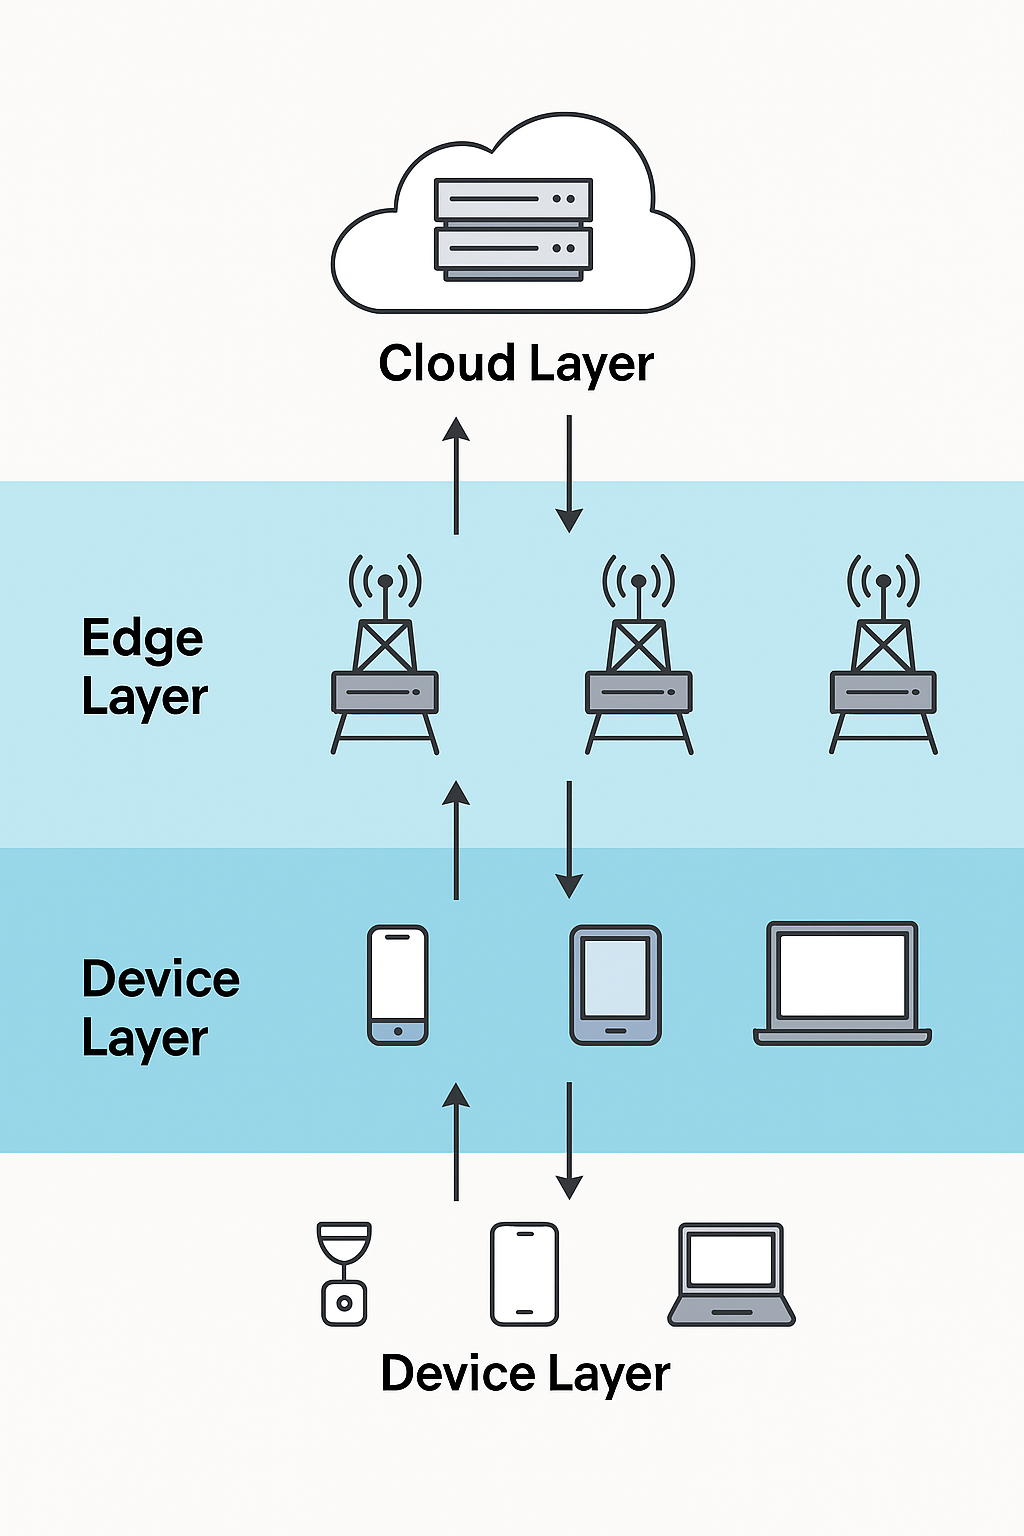
\includegraphics[width=0.9\linewidth]{mec_image.png}}
    \caption{Device layer, edge layer, and cloud layer network architecture.}
    \label{fig1}
\end{figure}

The system contains the following components:
\begin{itemize}
    \item Device layer: $\mathcal{D} = \{1, 2, ..., D\}$ represents $D = 20$ mobile devices, including low-end IoT devices (40\%, 0.2-0.5 GHz), mid-range mobile devices (40\%, 0.8-1.5 GHz), and high-end devices (20\%, 2.0-3.0 GHz)
    \item Edge layer: $\mathcal{E} = \{1, 2, ..., E\}$ represents $E = 4$ edge servers (4.0-6.0 GHz)
    \item Cloud layer: $\mathcal{C} = \{1, 2, ..., C\}$ represents $C = 2$ cloud servers (8.0-12.0 GHz)
    \item Task set: $\mathcal{T} = \{1, 2, ..., T\}$ represents $T = 40$ tasks to be processed, including compute-intensive (30\%), data-intensive (25\%), real-time sensitive (25\%), and lightweight (20\%)
\end{itemize}

\subsection{Computation Model}
\subsubsection{Task Characteristics}
Each task $i \in \mathcal{T}$ is characterized by a five-tuple:
\begin{equation}
\tau_i = (D_i, C_i, T_i^{\max}, \lambda_i, AoI_i^{\max})
\end{equation}
where:
\begin{itemize}
    \item $D_i$ is the input data size (MB), $D_i^{result}$ is the output data size
    \item $C_i$ is the computational complexity (CPU cycles/bit)
    \item $T_i^{\max}$ is the maximum tolerable delay (s)
    \item $\lambda_i$ is the task update interval (s)
    \item $AoI_i^{\max}$ is the maximum acceptable age of information (s)
\end{itemize}

\subsubsection{Delay Model}
The total task processing delay includes transmission delay, waiting delay, and computation delay:
\begin{equation}
T_i = T_i^{trans} + T_i^{wait} + T_i^{comp}
\end{equation}

Local execution delay only includes computation time:
\begin{equation}
T_{i,d(i)}^{local} = \frac{D_i \cdot C_i}{f_{i,d(i)}}
\end{equation}
where $f_{i,d(i)}$ is the CPU frequency allocated to task $i$.

The delay for offloading a task to an edge server:
\begin{equation}
T_{i,d(i),e(i)}^{edge} = \frac{D_i}{R_{d(i),e(i)}} + T_{queue}^{edge} + \frac{D_i \cdot C_i}{f_{i,e(i)}} + \frac{D_i^{result}}{R_{e(i),d(i)}}
\end{equation}
where $R_{j,k}$ is the transmission rate from node $j$ to $k$, calculated using Shannon's formula:
\begin{equation}
R_{j,k} = B_{j,k} \log_2\left(1 + \frac{P_j^{trans} \cdot h_{j,k}}{N_0 \cdot B_{j,k}}\right)
\end{equation}

\textbf{Queuing delay analysis}: Considering edge servers adopt the M/M/1 queuing model, the average waiting time is:
\begin{equation}
T_{queue}^{edge} = \frac{\rho}{f_e \cdot (1-\rho)}
\end{equation}
where $\rho = \lambda_e / \mu_e$ is the server utilization rate, $\lambda_e$ is the task arrival rate, and $\mu_e$ is the service rate.

\subsubsection{Energy Model}
Computation energy consumption adopts a dynamic power model:
\begin{equation}
E_{i,j}^{comp} = \kappa_j \cdot (f_{i,j})^{\alpha} \cdot D_i \cdot C_i
\end{equation}
where $\kappa_j \in [1.0, 3.5] \times 10^{-27}$ and $\alpha \in [2.2, 2.8]$ are set according to device type.

Transmission energy consumption: $E_{i,j,k}^{trans} = P_j^{trans} \cdot (D_i + D_i^{result})/R_{j,k}$, where $P_j^{trans} \in [0.1, 0.5]$ W.

The total energy consumption of mobile devices:
\begin{equation}
    \begin{split}
        E_i = x_{i}^{local} \cdot E_{i,d(i)}^{comp} + x_{i}^{edge} \cdot E_{i,d(i),e(i)}^{trans} \\ + x_{i}^{cloud} \cdot (E_{i,d(i),e(i)}^{trans} + E_{i,e(i),c(i)}^{trans})
    \end{split}
\end{equation}

\subsubsection{AoI Model}
To describe the freshness of information, we define the Age of Information (AoI) metric. For task $i$, its AoI at time $t$ is defined as:
\begin{equation}
AoI_i(t) = t - U_i(t)
\end{equation}
where $U_i(t)$ is the time when task $i$ last successfully completed an update.

Considering task processing delay and update interval, the average AoI of task $i$ is:
\begin{equation}
\overline{AoI}_i = \lambda_i + \frac{T_i}{2} + \frac{T_i^2}{2\lambda_i}
\end{equation}

This formula considers three parts: update interval $\lambda_i$, average waiting time $T_i/2$, and additional aging due to processing delay $T_i^2/(2\lambda_i)$.

\subsection{Optimization Problem Modeling}
\subsubsection{Decision Variables}
We define binary decision variables $\mathbf{x} = \{x_i^{local}, x_i^{edge}, x_i^{cloud}\}_{i \in \mathcal{T}}$, where:
\begin{itemize}
    \item $x_{i}^{local}$ indicates task $i$ is executed locally on the device
    \item $x_{i}^{edge}$ indicates task $i$ is offloaded to an edge server
    \item $x_{i}^{cloud}$ indicates task $i$ is offloaded to a cloud server
\end{itemize}
Continuous decision variables $\mathbf{f} = \{f_{i,j}\}_{i \in \mathcal{T}, j \in \mathcal{D} \cup \mathcal{E} \cup \mathcal{C}}$ represent the allocated CPU frequency.

\subsubsection{Objective Function}
Based on practical application requirements and recent research trends, we use the weighted sum method to transform the tri-objective into a single objective:
\begin{equation}
    \begin{split}
        \min_{\mathbf{x}, \mathbf{f}} F = \sum_{i \in \mathcal{T}} \bigg( w^E \cdot \frac{E_i}{E^{norm}} + w^T \cdot \frac{T_i}{T^{norm}}
        \\+ w^{AoI} \cdot \frac{\overline{AoI}_i}{AoI^{norm}} \bigg)
    \end{split}
\end{equation}
where:
\begin{itemize}
    \item Weight settings: $w^E = 0.25$, $w^T = 0.35$, $w^{AoI} = 0.40$ (prioritizing information timeliness)
    \item Normalization factors: $E^{norm} = \max_{i \in \mathcal{T}} E_i^{local}$, $T^{norm} = \max_{i \in \mathcal{T}} T_i^{cloud}$, $AoI^{norm} = \max_{i \in \mathcal{T}} AoI_i^{\max}$
\end{itemize}

\subsubsection{Constraints}
The main constraints include:
(1) Task allocation uniqueness: $x_{i}^{local} + x_{i}^{edge} + x_{i}^{cloud} = 1, \forall i$;
(2) Resource capacity: $\sum_{i} x_{i}^{j} \cdot f_{i,j} \leq F_{j}^{\max}$;
(3) Delay constraint: $T_i \leq T_i^{\max}$;
(4) AoI constraint: $\overline{AoI}_i \leq AoI_i^{\max}$;
(5) QoS constraint: 95\% of tasks meet delay requirements.

\subsubsection{Problem Complexity Analysis}
\textbf{Theorem 1}: The MEC task offloading and resource allocation problem considering AoI is NP-hard.

\textit{Proof}: Consider a special instance: only one edge server ($E = 1$), all tasks have the same data size $D$ and computational complexity $C$, and transmission delay and AoI constraints are ignored. In this case, the problem is equivalent to:
\begin{equation}
    \begin{split}
        \min_{S \subseteq \mathcal{T}} \sum_{i \in S} p_i, \quad
        \text{s.t.} \quad p_i = \frac{DC}{f_i}, \forall i \in S, \\
        \quad
        \sum_{i \in S} f_i \leq F^{\max}, \quad
        f_i \geq 0, \forall i \in S
    \end{split}
\end{equation}
where $S$ is the set of tasks selected for edge execution, and $F^{\max}$ is the total available CPU cycles of the server.

Define the "weight" $w_i = f_i$ and "value" $v_i$ for each task $i$ as:
\begin{equation}
v_i = \frac{1}{p_i} = \frac{f_i}{DC}
\end{equation}
Then equation (14) transforms into the classic Knapsack problem of selecting items in a knapsack with capacity $F^{\max}$ to maximize total value, which has been proven to be NP-hard.

Furthermore, the complete model contains both binary variables $\mathbf{x}$ and continuous variables $\mathbf{f}$, and the objective function includes nonlinear terms (such as $f_i^{\alpha}$), while also needing to consider the temporal dependencies of AoI constraints. Therefore, it belongs to Mixed Integer Nonlinear Programming (MINLP), making the solution even more difficult. $\square$

\section{TLBO-HHO Fusion Algorithm Design}
\subsection{Algorithm Motivation and Innovative Design Philosophy}
TLBO achieves stable population evolution through teacher-student interaction mechanism, while HHO realizes dynamic search by simulating hawk swarm hunting behavior. The proposed TLBO-HHO fusion algorithm adopts a two-phase integrated architecture: (1) two-phase collaborative mechanism, with TLBO guiding global exploration and HHO providing local exploitation; (2) adaptive parameter coordination; (3) AoI-aware constraint handling.

\subsection{Solution Encoding and Initialization}
Each solution $S_k$ is encoded as a mixed vector: $S_k = [\mathbf{x}_k, \mathbf{f}_k, \mathbf{a}_k]$, where $x_i^k \in \{0, 1, 2\}$ represents task execution location, $f_i^k$ is CPU frequency, and $a_i^k$ is server allocation. We adopt an intelligent initialization strategy with 30\% heuristic and 70\% random.

\begin{algorithm}[!b]
  \small
  \caption{Intelligent Initialization Strategy}
  \label{alg:init}
  \begin{algorithmic}[1]
    \REQUIRE Population size $P$
    \ENSURE Initialized population $\mathcal{P}$
    \STATE $\mathcal{P} \leftarrow \emptyset$
    \STATE $n_{heur} \leftarrow \lfloor 0.3 \times P \rfloor$ // Heuristic part
    \FOR{$i = 1$ \TO $n_{heur}$}
        \STATE $s \leftarrow \textsc{HeuristicInit}()$
        \STATE $\mathcal{P} \leftarrow \mathcal{P} \cup \{s\}$
    \ENDFOR
    \STATE $n_{rand} \leftarrow P - n_{heur}$ // Random part
    \FOR{$i = 1$ \TO $n_{rand}$}
        \STATE $s \leftarrow \textsc{RandomInit}()$
        \STATE $\mathcal{P} \leftarrow \mathcal{P} \cup \{s\}$
    \ENDFOR
    \RETURN $\mathcal{P}$
  \end{algorithmic}
\end{algorithm}

\subsection{Improved TLBO and HHO Mechanisms}
TLBO adopts an adaptive teaching factor: $T_F = 1 + rand() \cdot (1 + e^{-\sigma_{pop}/\sigma_{max}})$, and the enhanced teacher phase considers the influence of elite individuals. HHO introduces nonlinear escape energy: $E = 2E_0 \cdot \cos(\pi t/2T_{max}) \cdot (1 + 0.1 \sin(4\pi t/T_{max}))$, avoiding premature convergence (see Algorithm~\ref{alg:tlbo_hho_aoi}).

\subsection{Two-Phase Integration and AoI Optimization}
Adaptive probability switching: $p_{HHO} = p_{base} \cdot \alpha_{conv} \cdot \beta_{div}$, where $p_{base} = 0.7 - 0.6(t/T_{max})$. AoI-aware fitness function:
\begin{equation}
    \begin{split}
        Fitness(X) = w^E \cdot E(X) + w^T \cdot D(X) \\ 
        + w^{AoI} \cdot AoI(X) + Penalty(X)
    \end{split}
\end{equation}

\begin{algorithm}[!t]
  \small
  \caption{TLBO-HHO Two-Phase Integration Algorithm (with AoI Optimization)}
  \label{alg:tlbo_hho_aoi}
  \begin{algorithmic}[1]
    \REQUIRE Population size $N$, Maximum iterations $T_{\max}$, Weights $w^E, w^T, w^{AoI}$
    \ENSURE Optimal solution $\mathbf{X}_{best}$
    \STATE $P \leftarrow \textsc{IntelligentInit}(N)$; $ElitePool \leftarrow \emptyset$
    \STATE Evaluate all individual fitness (including AoI)
    \FOR{$t = 1$ \TO $T_{\max}$}
        \STATE $p_{HHO} \leftarrow \textsc{AdaptiveProb}(t, P)$
        \STATE $E \leftarrow \textsc{EscapeEnergy}(t)$; $T_F \leftarrow \textsc{TeachingFactor}(P)$
        \FOR{\textbf{each} $\mathbf{X}_i \in P$}
            \IF{$rand() < p_{HHO}$}
                \IF{$|E| \geq 1$}
                    \STATE $\mathbf{X}_{new} \leftarrow \textsc{HHO\_Explore}(\mathbf{X}_i, \mathbf{X}_{best})$
                \ELSE
                    \STATE $\mathbf{X}_{new} \leftarrow \textsc{HHO\_Exploit}(\mathbf{X}_i, \mathbf{X}_{best}, E, J)$
                \ENDIF
            \ELSE
                \STATE $\mathbf{X}_{teacher} \leftarrow \textsc{SelectTeacher}(P, ElitePool)$
                \STATE $\mathbf{X}_{new} \leftarrow \textsc{TLBO\_Teach}(\mathbf{X}_i, \mathbf{X}_{teacher}, T_F)$
                \STATE $\mathbf{X}_{new} \leftarrow \textsc{TLBO\_Learn}(\mathbf{X}_{new}, P)$
            \ENDIF
            \STATE $\mathbf{X}_{new} \leftarrow \textsc{ConstraintRepair}(\mathbf{X}_{new})$
            \STATE $f_{new} \leftarrow \textsc{Evaluate}(\mathbf{X}_{new}) + \textsc{Penalty}(\mathbf{X}_{new})$
            \IF{$f_{new} < f(\mathbf{X}_i)$}
                \STATE $\mathbf{X}_i \leftarrow \mathbf{X}_{new}$; Update $ElitePool$
            \ENDIF
        \ENDFOR
    \ENDFOR
    \RETURN $\mathbf{X}_{best}$
  \end{algorithmic}
\end{algorithm}

\section{Experiments and Results Analysis}
\subsection{Experimental Setup}
\subsubsection{MEC System Parameter Configuration}
Based on actual MEC deployment scenarios and configurations of AWS Wavelength and Azure Edge Zones, the parameters are set as shown in Table~\ref{tab:system}.

\begin{table}[!b]
\small
\centering
\caption{MEC System Parameter Configuration}
\label{tab:system}
\begin{tabular}{|l|l|}
\hline
Parameter & Value \\
\hline
Number of devices/edge/cloud servers & 20/4/2 \\
Device/edge/cloud CPU frequency & 0.2-3/4-6/8-12 GHz \\
Transmission power range & 0.1-0.5 W \\
Bandwidth (device-edge/edge-cloud) & 10-50/100-1000 Mbps \\
\hline
\end{tabular}
\end{table}

% \begin{table}[H]
%   \scriptsize
%   \setlength{\tabcolsep}{4pt}
%   \centering
%   \caption{任务类型分布及其特征}
%   \label{tab:task}

%   \resizebox{\columnwidth}{!}{%
%     \begin{tabular}{|l|c|c|c|c|}
%       \hline
%       任务类型 & 数量(\%) & 平均负载(G) & 更新间隔(s) & 最大AoI(s) \\
%       \hline
%       计算密集型 & 30 & 1.36 & 0.949 & 2.549 \\
%       数据密集型 & 25 & 3.23 & 1.214 & 4.114 \\
%       实时敏感型 & 25 & 0.14 & 0.617 & 0.690 \\
%       轻量级     & 20 & 0.01 & 1.302 & 1.619 \\
%       \hline
%     \end{tabular}}
% \end{table}

\begin{table}[!b]
  \scriptsize
  \setlength{\tabcolsep}{4pt}
  \centering
  \caption{Task Type Distribution and Characteristics}
  \label{tab:task}
  \resizebox{\columnwidth}{!}{%
    \begin{tabular}{|l|c|c|c|c|}
       \hline
        Task Type & Ratio(\%) & Avg Load(G) & Update Int.(s) & Max AoI(s) \\
        \hline
        Compute-intensive & 30 & 1.36 & 0.949 & 2.549 \\
        Data-intensive & 25 & 3.23 & 1.214 & 4.114 \\
        Real-time sensitive & 25 & 0.14 & 0.617 & 0.690 \\
        Lightweight & 20 & 0.01 & 1.302 & 1.619 \\
        \hline
    \end{tabular}}
  % \begin{tabular}{|l|c|c|c|c|}
  %   \hline
  %   Task Type & Ratio(\%) & Avg Load(G) & Update Int.(s) & Max AoI(s) \\
  %   \hline
  %   Compute-intensive & 30 & 1.36 & 0.949 & 2.549 \\
  %   Data-intensive & 25 & 3.23 & 1.214 & 4.114 \\
  %   Real-time sensitive & 25 & 0.14 & 0.617 & 0.690 \\
  %   Lightweight & 20 & 0.01 & 1.302 & 1.619 \\
  %   \hline
  % \end{tabular}
\end{table}

\subsubsection{Algorithm Parameter Settings}
The optimal parameter configuration was determined through orthogonal experiments and grid search. Common parameters: population size 50, maximum iterations 150, 5 independent runs, weight settings $w^E = 0.25$, $w^T = 0.35$, and $w^{AoI} = 0.40$. TLBO-HHO specific parameters include: initial HHO probability $p_{max} = 0.7$, final HHO probability $p_{min} = 0.1$, elite pool ratio 10\%.

\subsection{Algorithm Convergence Analysis}
Fig.~\ref{fig:convergence} shows the convergence curve comparison of the four algorithms. TLBO-HHO drops rapidly in the initial phase (0-25 iterations), maintains stable improvement in the middle phase, and finally converges to 0.00102. In contrast, TLBO converges stably but slowly (0.00292), GA easily falls into local optima (0.00757), and GWO performs poorly (0.00367).

\begin{figure}[!b]
    \centering
    \centerline{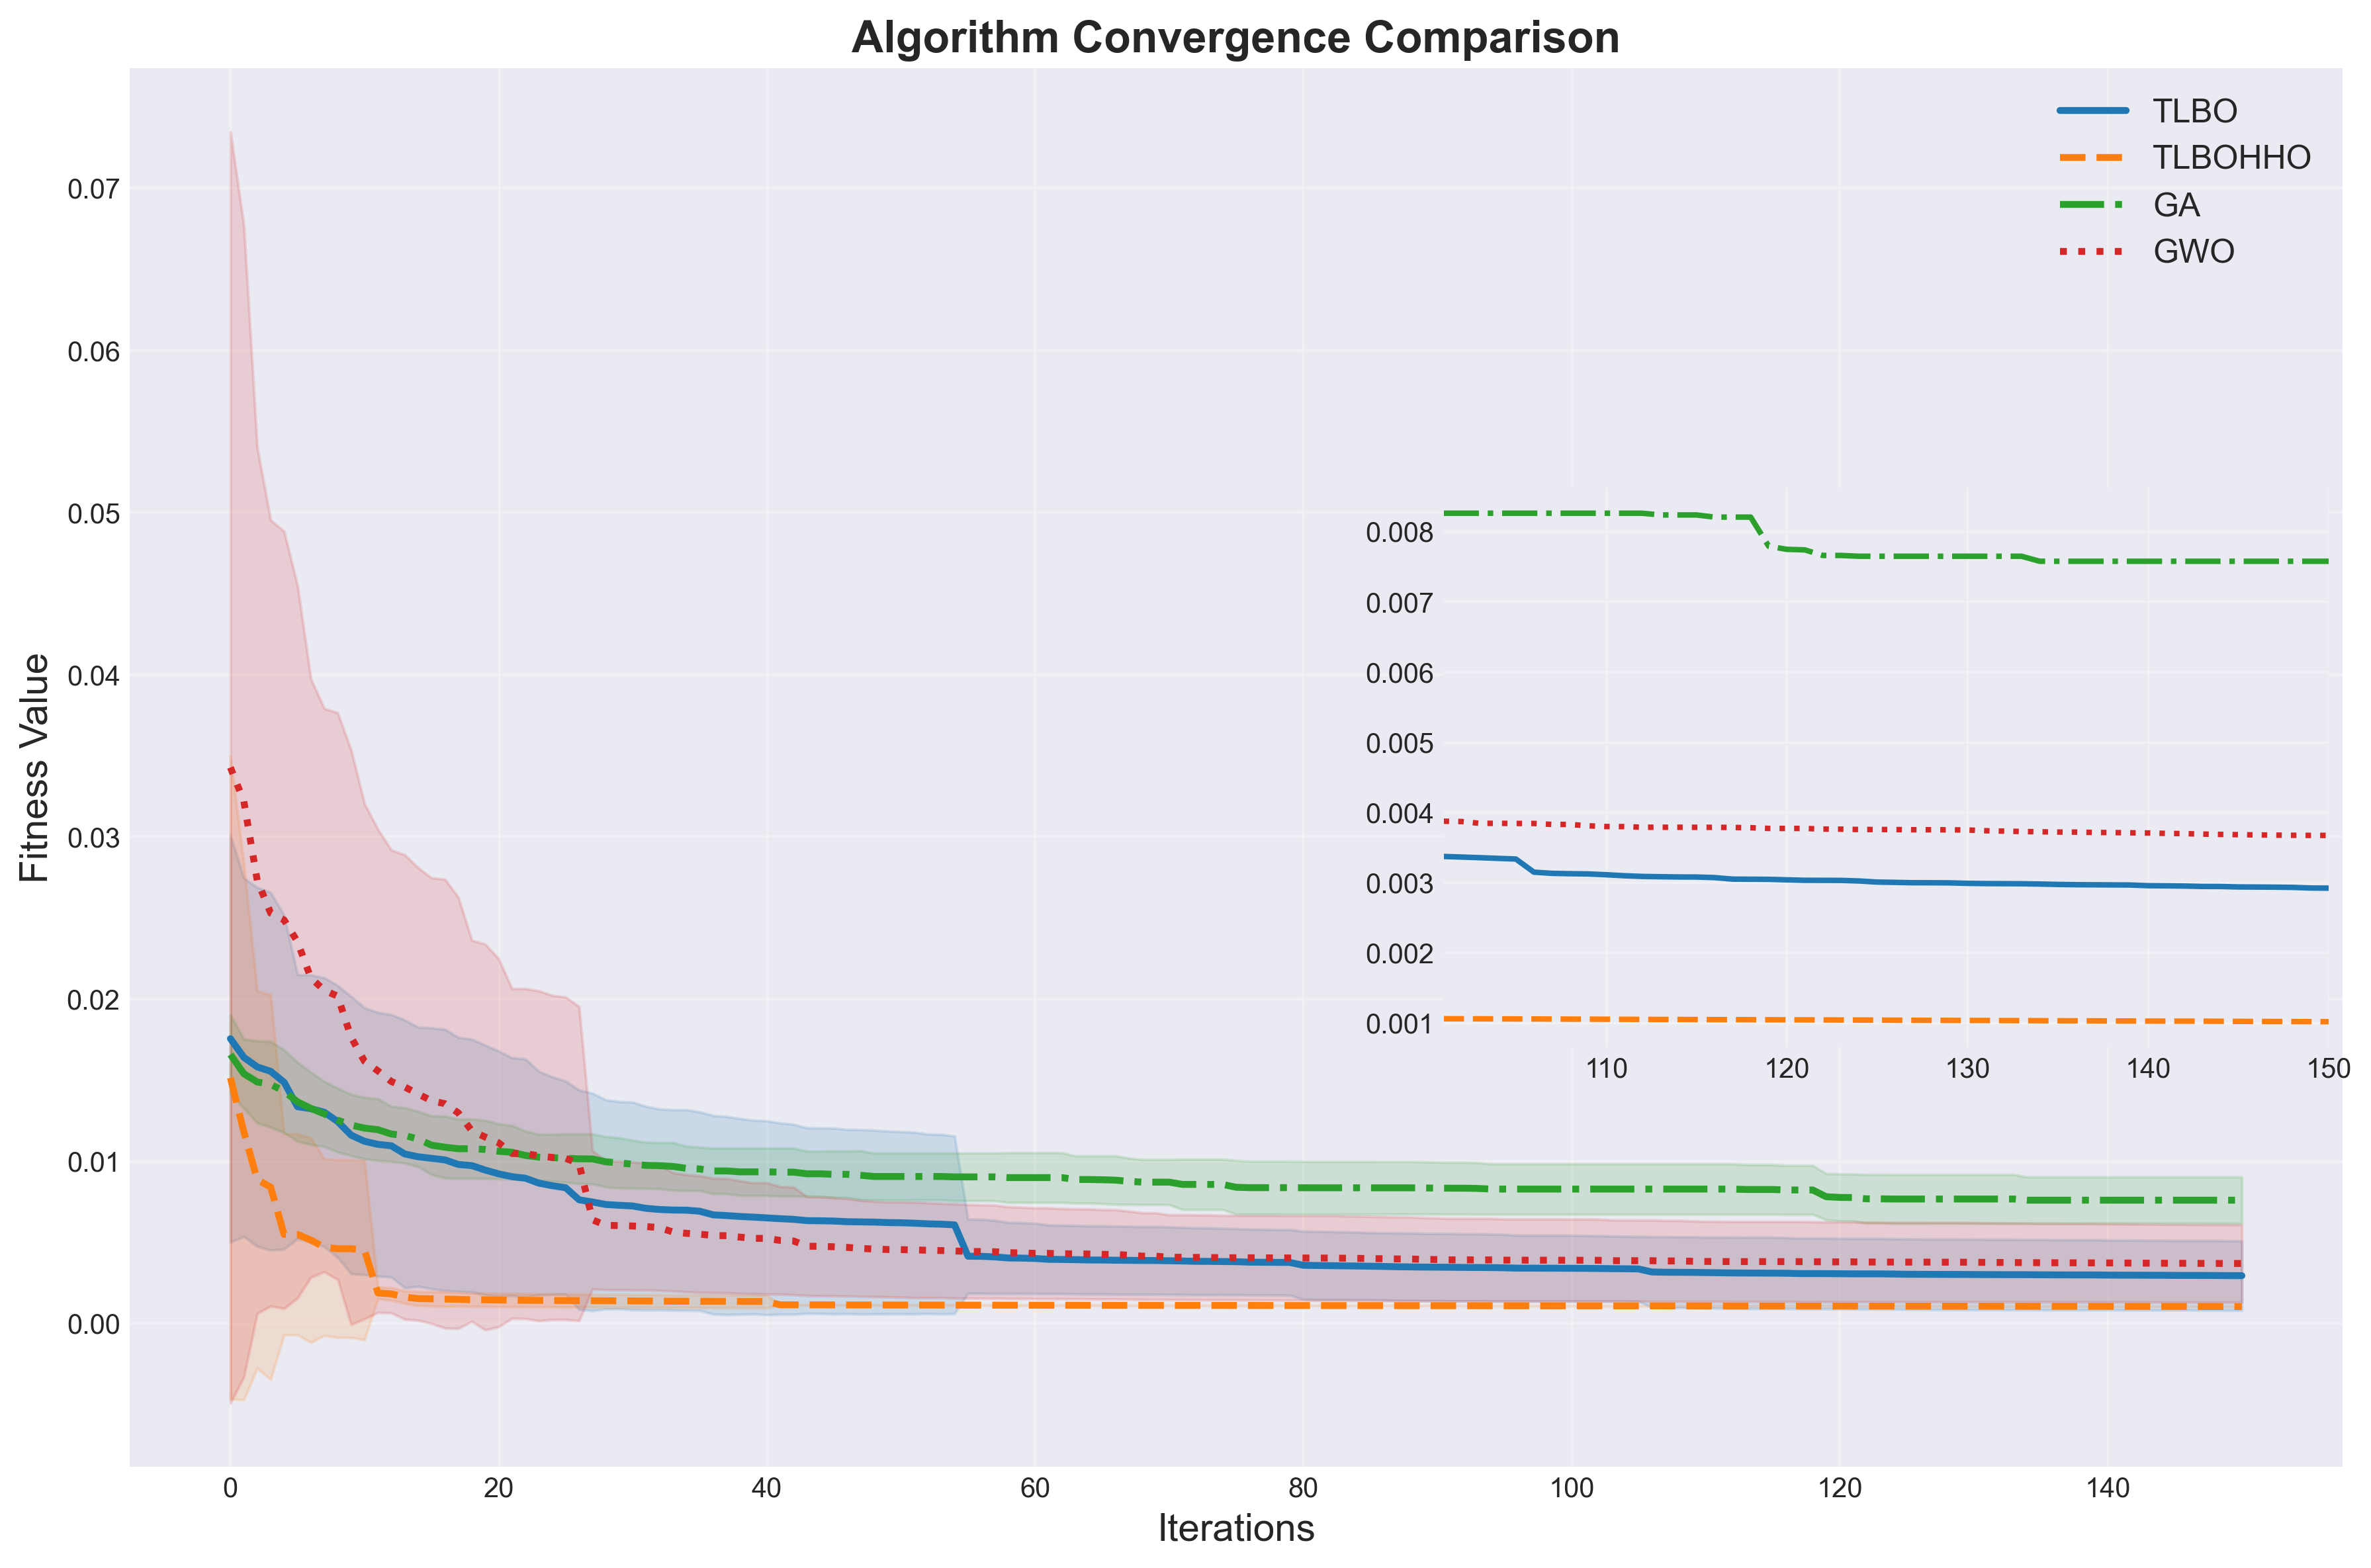
\includegraphics[width=0.9\linewidth]{convergence_comparison.png}}
    \caption{Algorithm convergence curve comparison}
    \label{fig:convergence}
\end{figure}

\subsection{Performance Comparison Analysis}
Fig.~\ref{fig:metrics} shows the performance metrics comparison of the four algorithms. TLBO-HHO achieves an average fitness of 0.00102, improving by 65.2\%, 85.4\%, and 74.6\% compared to TLBO, GA, and GWO respectively. In terms of energy consumption, TLBO-HHO only consumes 3.19J, significantly lower than GA (31.14J). Although GA achieves the best delay (0.577s), its energy consumption is too high; GWO has the fewest AoI violations (4.6 times), but its overall performance is inferior to TLBO-HHO.

\begin{figure}[!t]
    \centering
    \centerline{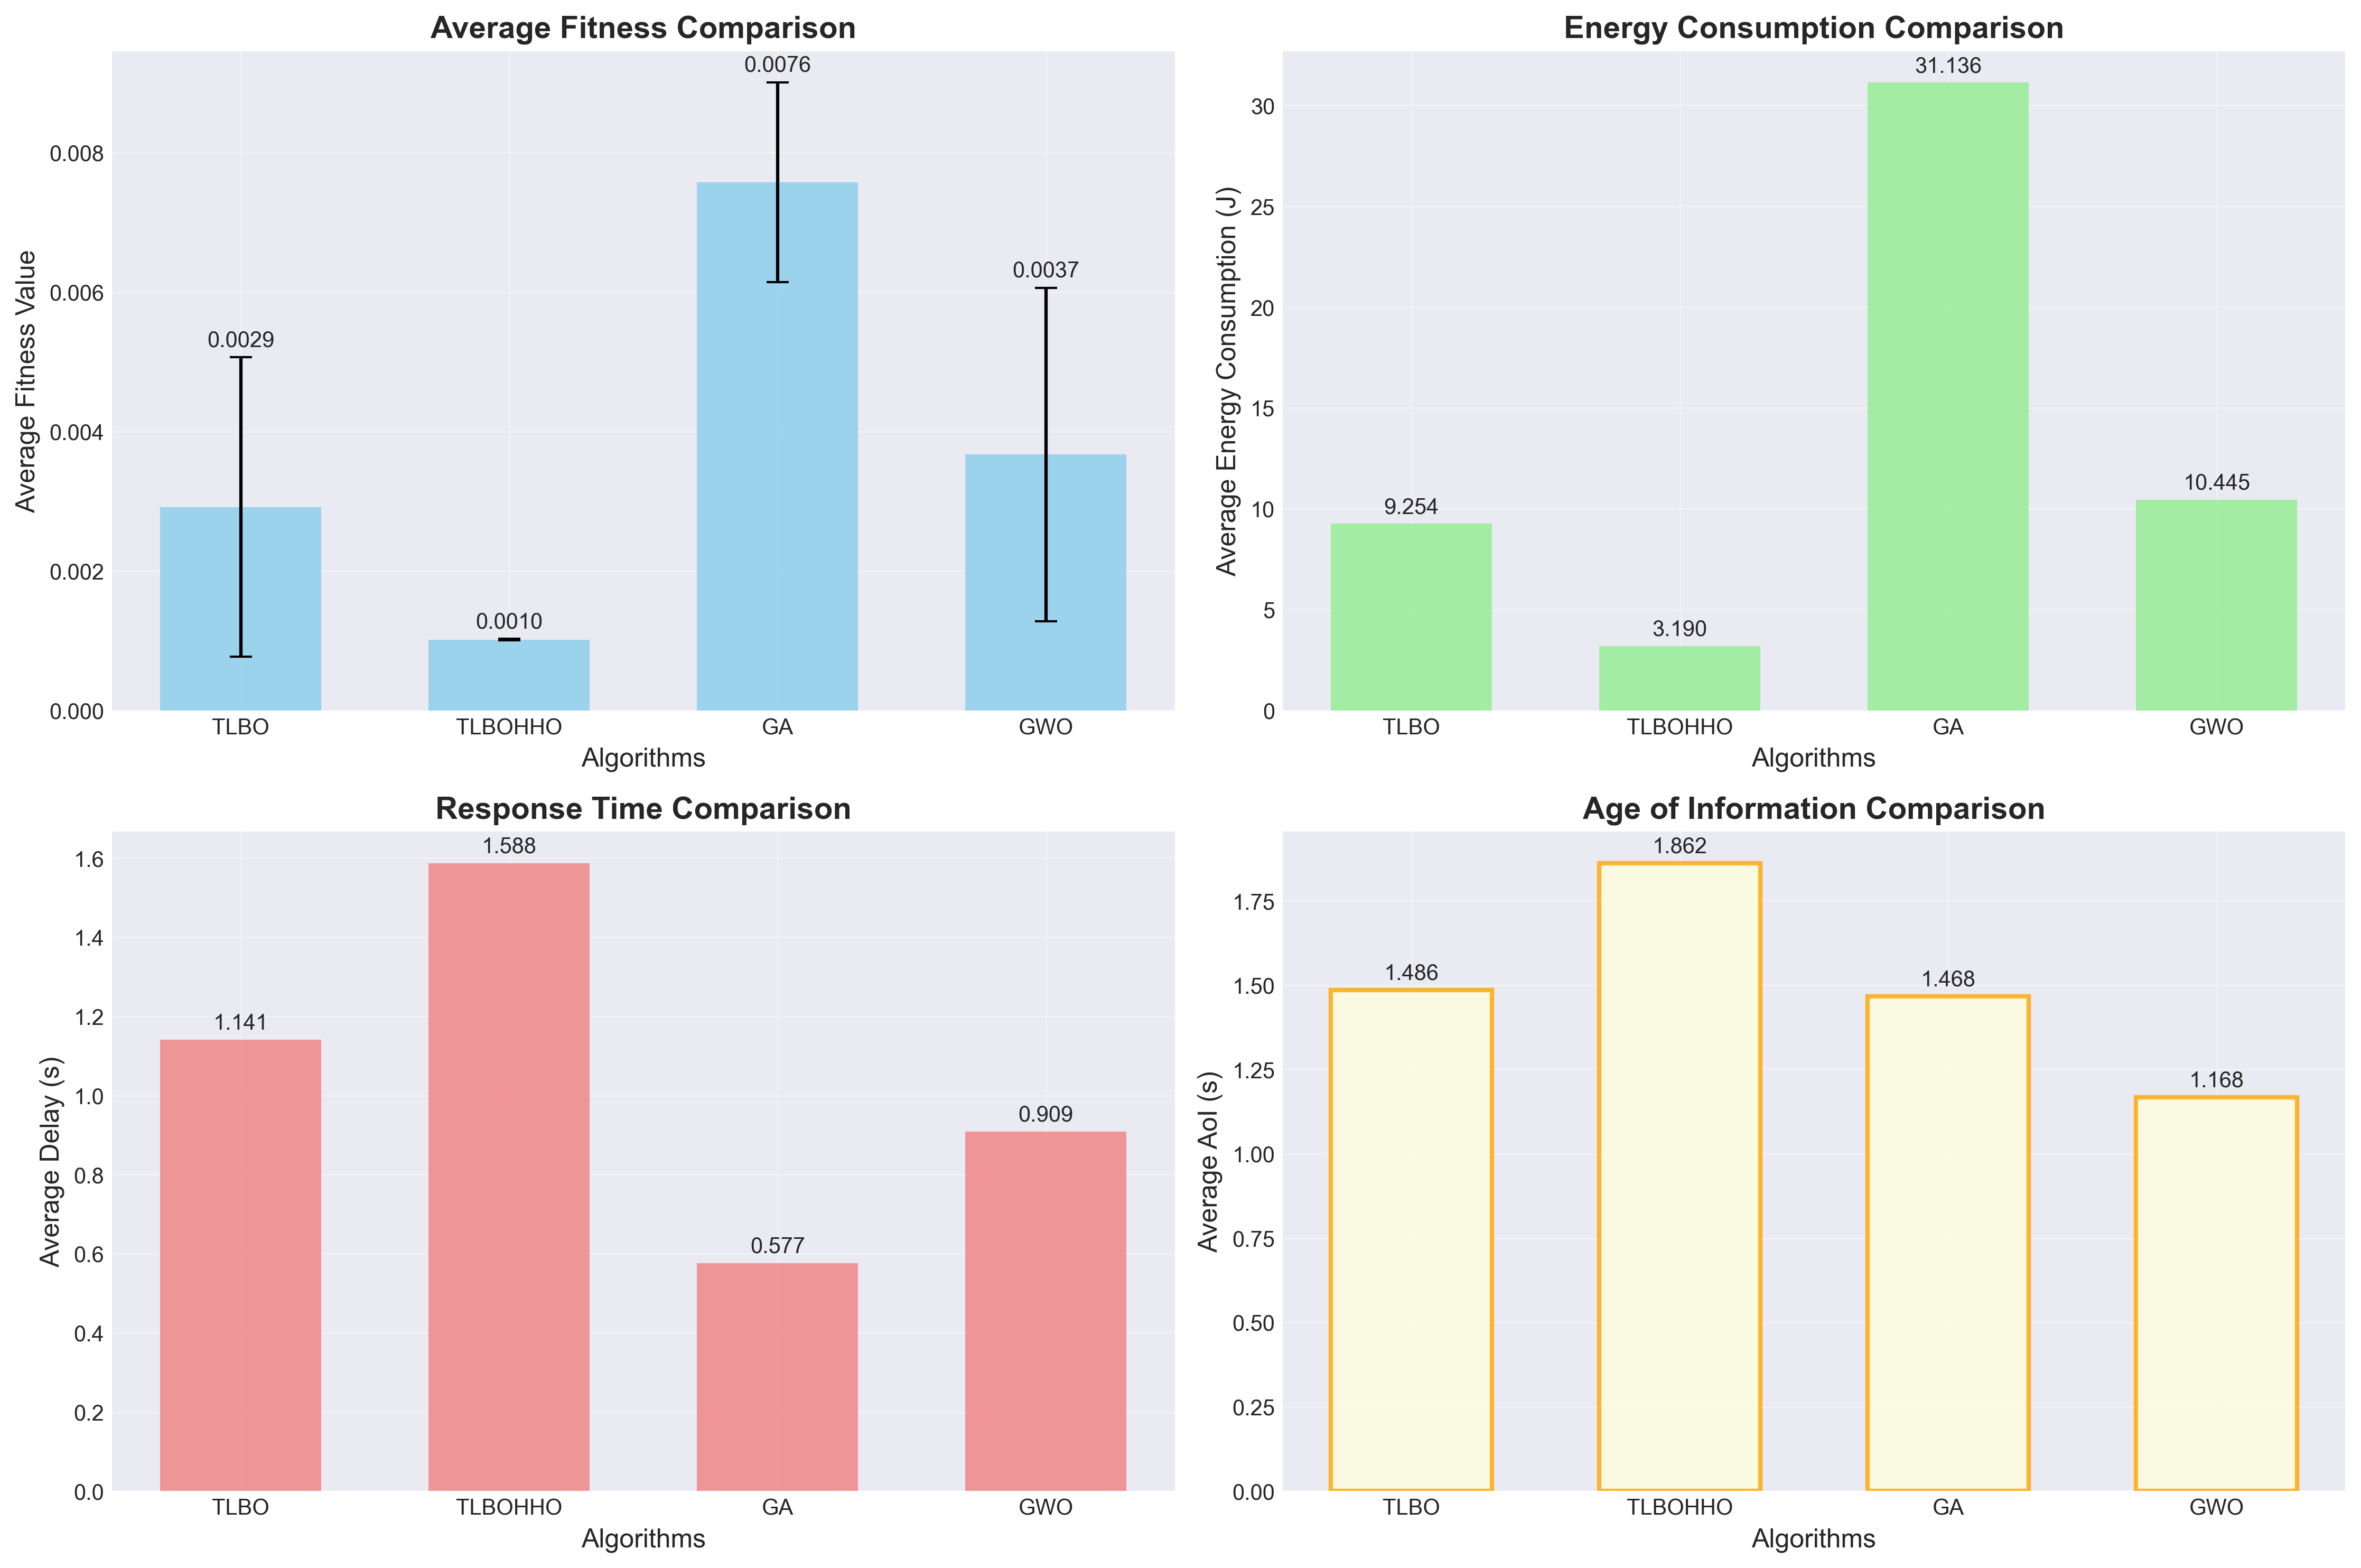
\includegraphics[width=0.9\linewidth]{performance_metrics_detail.png}}
    \caption{Algorithm performance metrics comparison}
    \label{fig:metrics}
\end{figure}

\subsection{Task Allocation Strategy Analysis}
Fig.~\ref{fig:allocation} shows the task allocation location comparison. TLBO-HHO adopts a highly localized strategy (97.5\% local execution), effectively reducing transmission delay and energy consumption. In contrast, GA overuses edge resources (22.5\%), and GWO has the highest cloud utilization (12.5\%).

\begin{figure}[!b]
    \centering
    \centerline{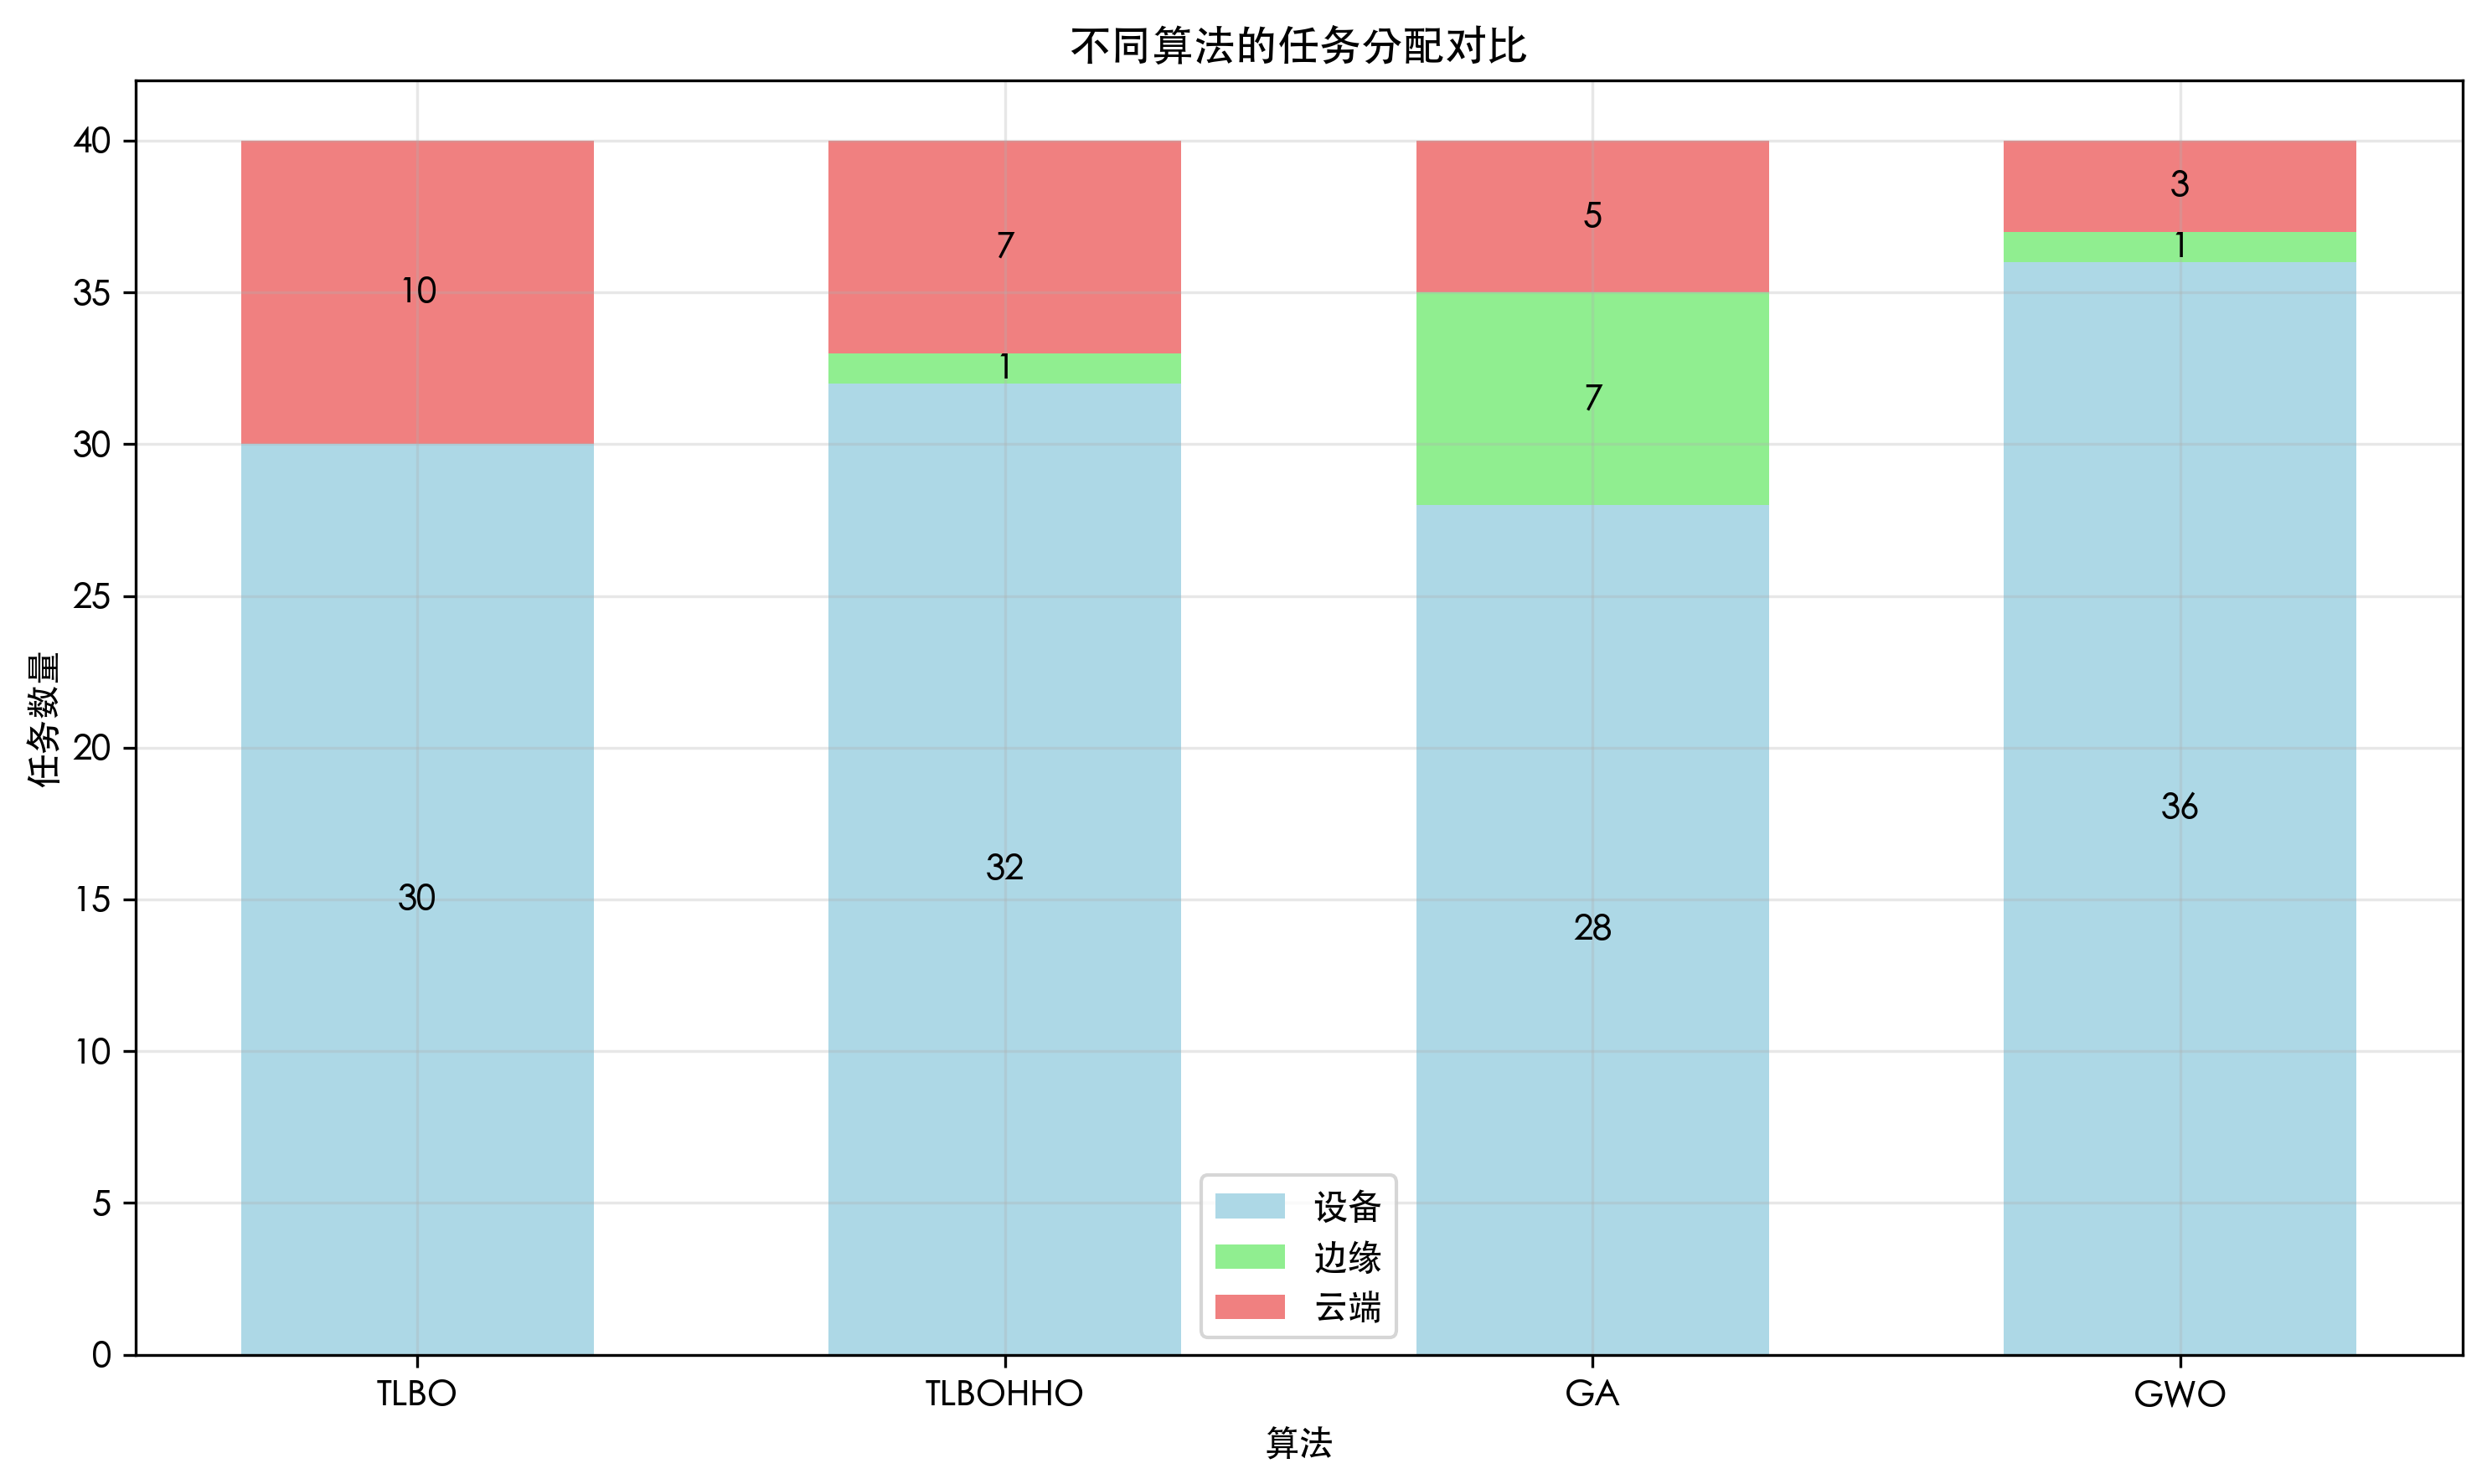
\includegraphics[width=0.9\linewidth]{task_allocation_comparison.png}}
    \caption{Algorithm task allocation comparison}
    \label{fig:allocation}
\end{figure}

\subsection{AoI Performance Analysis}
Fig.~\ref{fig:aoi_analysis} shows the AoI performance for different task types. TLBO-HHO performs best for real-time sensitive tasks, with 95\% of AoI within 1 second. Through prioritized local execution and reasonable resource allocation, the AoI of all task types remains within acceptable ranges.

\begin{figure}[!b]
    \centering
    \centerline{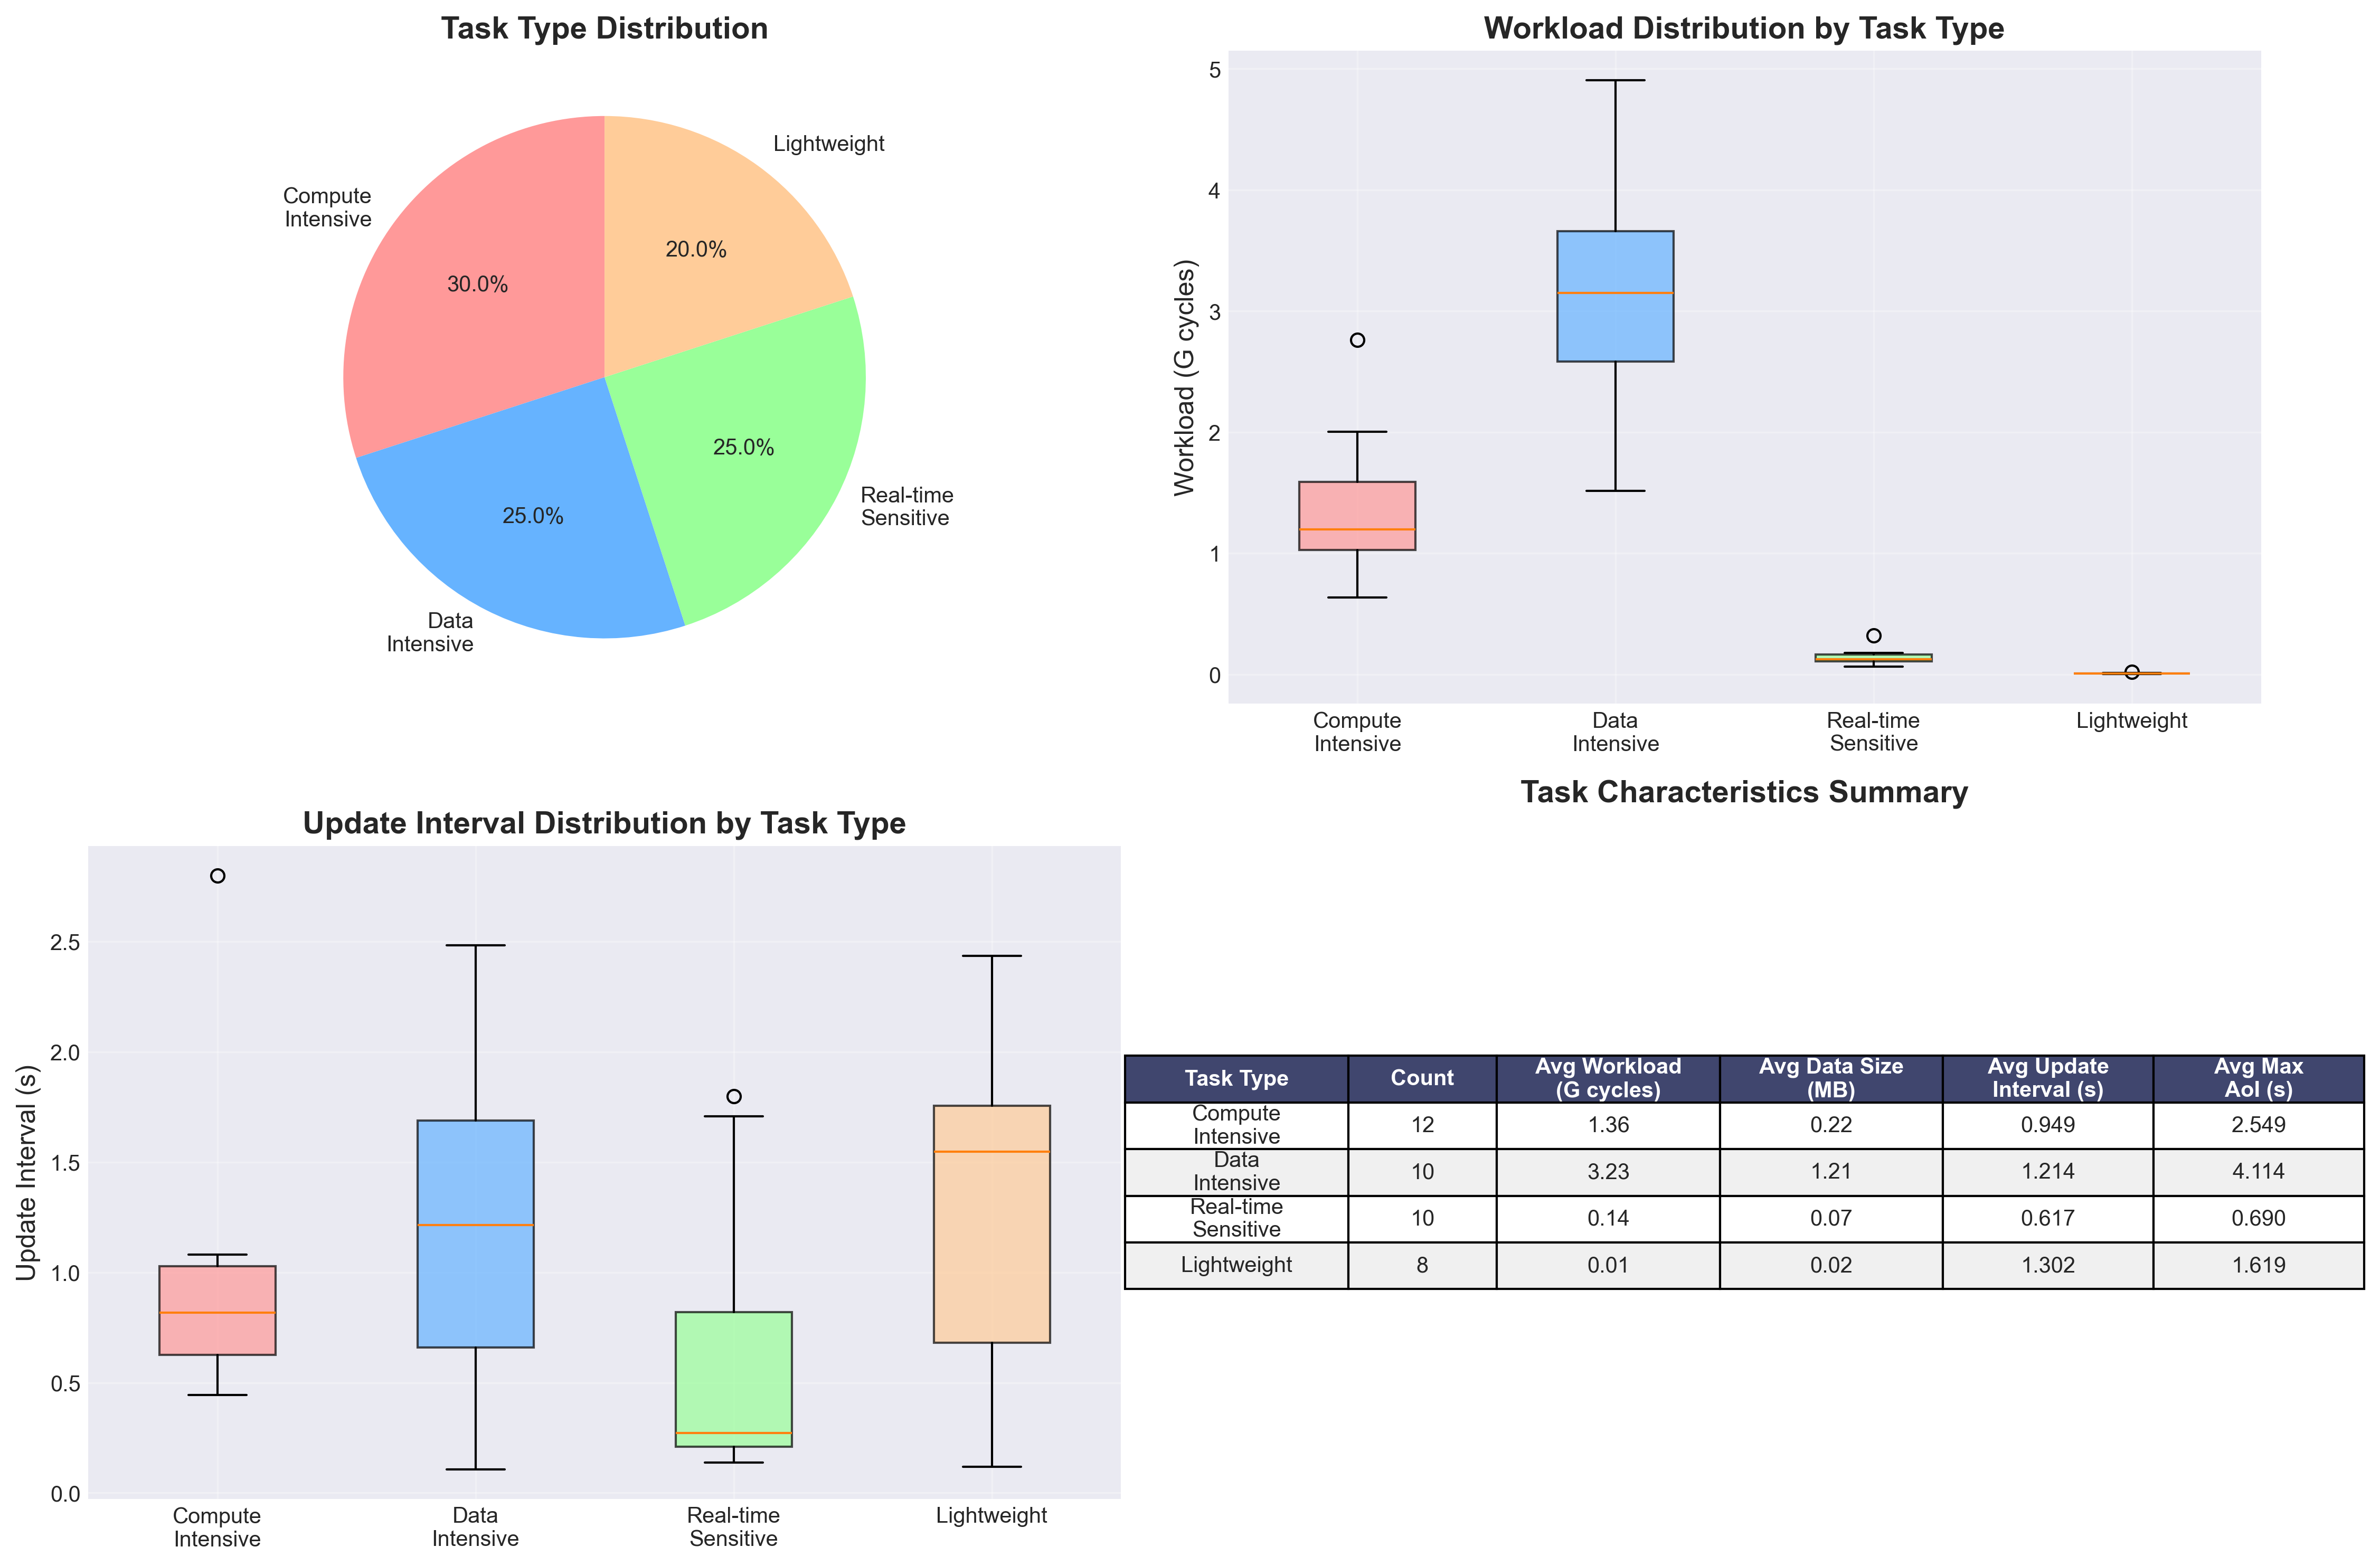
\includegraphics[width=0.9\linewidth]{task_type_characteristics.png}}
    \caption{Task type AoI performance analysis}
    \label{fig:aoi_analysis}
\end{figure}

\section{Conclusion and Future Work}
\subsection{Research Summary}
This paper addresses the task offloading and resource allocation optimization problem in mobile edge computing, proposing a two-phase integrated TLBO-HHO fusion algorithm that incorporates AoI into MEC task offloading optimization for the first time. Through theoretical analysis, algorithm design, and experimental validation, we draw the following conclusions:

\textbf{Problem modeling contribution}: We established a tri-objective optimization model considering energy consumption, delay, and AoI, with weight settings of 0.25-0.35-0.40 to adapt to information timeliness requirements. We analyzed task waiting time through queuing theory and proved the NP-hard nature of the problem through theoretical proof, providing a theoretical basis for adopting metaheuristic algorithms. The model considers multi-dimensional constraints of actual MEC systems, including resource capacity, bandwidth limitations, delay requirements, energy budget, and AoI constraints, making it closer to practical application scenarios.

\textbf{Algorithm design innovation}: The proposed two-phase integrated TLBO-HHO algorithm achieves performance breakthrough through innovative fusion mechanisms. The algorithm uses TLBO's teaching phase to guide global exploration and HHO's hunting strategy to provide local exploitation, achieving dynamic balance between exploration and exploitation through adaptive probability switching (0.7$\rightarrow$0.1) and parameter coordination strategies. In particular, the introduced AoI-aware fitness evaluation and constraint handling mechanisms enable the algorithm to effectively optimize information freshness.

\textbf{Significant performance improvement}: In an experimental scenario containing 20 devices, 4 edge servers, 2 cloud servers, and 40 tasks, TLBO-HHO achieved fitness value improvements of 65.2\%, 85.4\%, and 74.6\% compared to TLBO, GA, and GWO respectively. The algorithm performs particularly well in energy consumption, with an average energy consumption of only 3.19J, 89.8\% lower than GA. Meanwhile, through a 97.5\% local execution strategy, it effectively balances delay and AoI performance.

\textbf{Practical application value}: The algorithm demonstrates intelligent task allocation strategies that can adaptively adjust execution locations according to task types. For real-time sensitive tasks, 95\% of AoI is controlled within 1 second; for compute-intensive tasks, performance is guaranteed through reasonable resource allocation. This differentiated processing strategy meets the requirements of actual MEC applications and has important practical value.

\subsection{Research Limitations}
Despite achieving significant results, this research still has the following limitations:

\textbf{Static scenario assumption}: The current model assumes that task characteristics and network states are relatively stable, without fully considering user mobility, channel time-variability, and dynamic task arrivals. In actual MEC systems, these dynamic factors have important impacts on performance.

\textbf{Centralized decision architecture}: The algorithm adopts centralized optimization, requiring global information collection and computation. In large-scale distributed MEC scenarios, it may face issues such as high communication overhead, single point of failure, and limited scalability.

\textbf{Insufficient security considerations}: The data privacy protection, communication security, and malicious attack defense during task offloading are not fully considered.

\textbf{Simplified AoI model}: The current AoI model assumes fixed task update intervals without considering random arrivals and non-periodic updates.

\subsection{Future Research Directions}
Based on this research and existing limitations, future research directions include:

\textbf{Distributed algorithm implementation}: Research on distributed versions of TLBO-HHO to reduce communication overhead, design consensus-based distributed optimization frameworks, and achieve collaborative optimization between edge nodes.

\textbf{Dynamic scenario extension}: Consider user mobility and dynamic task arrivals, design online optimization mechanisms, and research multi-timescale AoI optimization strategies.

\textbf{Federated learning integration}: Combine federated learning to protect user privacy, design privacy-preserving distributed task offloading mechanisms, and optimize AoI while ensuring data security.

\textbf{Multi-objective optimization deepening}: Research more complex multi-objective optimization frameworks, consider other objectives such as service quality and fairness, and design generation and selection mechanisms for Pareto optimal solution sets.

\textbf{Practical system deployment}: Validate algorithm performance on real MEC testbeds, consider actual network protocols and system overhead, and develop optimization tools for industrial applications.

\begin{thebibliography}{00}
\bibitem{b1} Y. Mao, C. You, J. Zhang, K. Huang, and K. B. Letaief, ``A survey on mobile edge computing: The communication perspective,'' \textit{IEEE Commun. Surveys Tuts.}, vol. 19, no. 4, pp. 2322--2358, 4th Quart., 2017.
\bibitem{b2} S. Sardellitti, G. Scutari, and S. Barbarossa, ``Joint optimization of radio and computational resources for multicell mobile-edge computing,'' \textit{IEEE Trans. Signal Inf. Process. Netw.}, vol. 1, no. 2, pp. 89--103, Jun. 2015.
\bibitem{b3} L. Huang, S. Bi, and Y. J. A. Zhang, ``Deep reinforcement learning for online computation offloading in wireless powered mobile-edge computing networks,'' \textit{IEEE Trans. Mobile Comput.}, vol. 19, no. 11, pp. 2581--2593, Nov. 2020.
\bibitem{b4} S. Guo, B. Xiao, Y. Yang, and Y. Yang, ``Energy-efficient dynamic offloading and resource scheduling in mobile cloud computing,'' in \textit{Proc. IEEE INFOCOM}, San Francisco, CA, USA, Apr. 2016, pp. 1--9.
\bibitem{b5} R. V. Rao, V. J. Savsani, and D. P. Vakharia, ``Teaching--learning-based optimization: A novel method for constrained mechanical design optimization problems,'' \textit{Comput.-Aided Des.}, vol. 43, no. 3, pp. 303--315, Mar. 2011.
\bibitem{b6} A. A. Heidari, S. Mirjalili, H. Faris, I. Aljarah, M. Mafarja, and H. Chen, ``Harris hawks optimization: Algorithm and applications,'' \textit{Future Gener. Comput. Syst.}, vol. 97, pp. 849--872, Aug. 2019.
\bibitem{b7} H. Chen, A. A. Heidari, H. Chen, M. Wang, Z. Pan, and A. H. Gandomi, ``Multi-population differential evolution-assisted Harris hawks optimization: Framework and case studies,'' \textit{Future Gener. Comput. Syst.}, vol. 111, pp. 175--198, Oct. 2020.
\bibitem{b8} B. Tu, F. Wang, Y. Huo, and X. Wang, ``A hybrid algorithm of grey wolf optimizer and harris hawks optimization for solving global optimization problems with improved convergence performance,'' \textit{Sci. Rep.}, vol. 13, no. 1, p. 22909, Dec. 2023.
\bibitem{b9} C. Wang, F. R. Yu, C. Liang, Q. Chen, and L. Tang, ``Joint computation offloading and interference management in wireless cellular networks with mobile edge computing,'' \textit{IEEE Trans. Veh. Technol.}, vol. 66, no. 8, pp. 7432--7445, Aug. 2017.
\bibitem{b10} J. Liu, Y. Mao, J. Zhang, and K. B. Letaief, ``Delay-optimal computation task scheduling for mobile-edge computing systems,'' in \textit{Proc. IEEE Int. Symp. Inf. Theory (ISIT)}, Barcelona, Spain, Jul. 2016, pp. 1451--1455.
\bibitem{b11} L. Wang, K. Wang, C. Pan, W. Xu, N. Aslam, and L. Hanzo, ``Deep reinforcement learning based dynamic trajectory control for UAV-assisted mobile edge computing,'' \textit{IEEE Trans. Mobile Comput.}, vol. 21, no. 10, pp. 3536--3550, Oct. 2022.
\bibitem{b12} Z. Li and Q. Zhu, ``Genetic algorithm-based optimization of offloading and resource allocation in mobile-edge computing,'' \textit{Information}, vol. 11, no. 2, p. 83, Feb. 2020.
\bibitem{b13} L. Zang, X. Zhang, and B. Guo, ``Federated deep reinforcement learning for online task offloading and resource allocation in WPC-MEC networks,'' \textit{IEEE Access}, vol. 10, pp. 9856--9867, 2022.
\bibitem{b14} A. Ali, S. A. A. Shah, T. Al Shloul, A. Khattak, A. Ahmad, and A. Ali, ``Multiobjective Harris Hawks optimization-based task scheduling in cloud-fog computing,'' \textit{IEEE Internet Things J.}, vol. 11, no. 13, pp. 24334--24352, Jul. 2024.
\bibitem{b15} M. A. Abd-Elmagid, N. Pappas, and H. S. Dhillon, ``On the role of age of information in the Internet of Things,'' \textit{IEEE Commun. Mag.}, vol. 57, no. 12, pp. 72--77, Dec. 2019.
\bibitem{b16} S. Kaul, R. Yates, and M. Gruteser, ``Real-time status: How often should one update?'' in \textit{Proc. IEEE INFOCOM}, Orlando, FL, USA, Mar. 2012, pp. 2731--2735.
\bibitem{b17} L. Liu, J. Feng, X. Mu, Q. Pei, D. Lan, and M. Xiao, ``Asynchronous deep reinforcement learning for collaborative task computing and on-demand resource allocation in vehicular edge computing,'' \textit{IEEE Trans. Intell. Transp. Syst.}, vol. 24, no. 12, pp. 15513--15526, Dec. 2023.
\bibitem{b18} Z. Zhou, P. Liu, J. Feng, Y. Zhang, S. Mumtaz, and J. Rodriguez, ``Computation resource allocation and task assignment optimization in vehicular fog computing: A contract-matching approach,'' \textit{IEEE Trans. Veh. Technol.}, vol. 68, no. 4, pp. 3113--3125, Apr. 2019.
\end{thebibliography}

\end{document}